% answers.tex —— 1990 年·广东卷·文史类 · 参考答案与详细解析片段
% 由 tools/generate_projects.py 依来源总账自 1990/1990_广东_试题.md + 1990/1990_广东_解析正文.md + 1990/1990_广东_答案要点.md 生成，勿手改（改源 MD 后重跑）


卷内第一卷只列代号，第二卷第一题只列结果、第二题给出详解，第三至五题仅注「见理工农医类」相应题号。以下按题整理：第一卷补出必要推导，第二卷第二题以卷内解法为主线重述，第三至五题给出完整推导。

第二卷大题卷面编号为一、二、三、四、五，本稿续编为第 26—30 题。

\gkpart{第一卷（第 1—25 题）}

\begin{answer}
\gksolhead{1}{}

\textbf{题目}：

如果 $0<\theta<\pi$，且 $\cos\theta=-\dfrac{\sqrt3}{2}$，那么 $\theta$ 等于（　）。

（A）$\frac{5\pi}{6}$；（B）$\frac{2\pi}{3}$；（C）$\frac{\pi}{3}$；（D）$\frac{\pi}{6}$。

\Needspace{4\baselineskip}
\textbf{解析}

\Needspace{5\baselineskip}
由 $0<\theta<\pi$ 且 $\cos\theta<0$，知 $\theta\in\left(\dfrac{\pi}{2},\pi\right)$。而

\nopagebreak[4]
\[
\cos\frac{5\pi}{6}=-\frac{\sqrt3}{2},
\]

故 $\theta=\dfrac{5\pi}{6}$。

\gkanswer{答案：A。}

\end{answer}
\begin{answer}
\gksolhead{2}{}

\textbf{题目}：

函数 $f(x)=\sqrt{1+2x}+\sqrt{1-2x}$ 的定义域是（　）。

（A）$\left(-\infty,-\frac12\right]$；（B）$\left[\frac12,+\infty\right)$；（C）$\left[-\frac12,+\infty\right)$；（D）$\left[-\frac12,\frac12\right]$。

\Needspace{4\baselineskip}
\textbf{解析}

\Needspace{5\baselineskip}
根号内须非负，即

\nopagebreak[4]
\[
1+2x\ge 0,\qquad 1-2x\ge 0.
\]

解得 $-\dfrac12\le x\le\dfrac12$，定义域为 $\left[-\dfrac12,\dfrac12\right]$。

\gkanswer{答案：D。}

\end{answer}
\begin{answer}
\gksolhead{3}{}

\textbf{题目}：

椭圆 $\dfrac{(x+1)^2}{16}+\dfrac{y^2}{25}=1$ 的离心率是（　）。

（A）$\frac35$；（B）$\frac34$；（C）$\frac{\sqrt{41}}{4}$；（D）$\frac{\sqrt{41}}{5}$。

\Needspace{4\baselineskip}
\textbf{解析}

\Needspace{5\baselineskip}
椭圆的长半轴 $a=5$（沿 $y$ 轴方向），短半轴 $b=4$，故

\nopagebreak[4]
\[
c=\sqrt{a^2-b^2}=\sqrt{25-16}=3,
\]

离心率 $e=\dfrac{c}{a}=\dfrac35$。中心平移到 $(-1,0)$ 不改变离心率。

\gkanswer{答案：A。}

\end{answer}
\begin{answer}
\gksolhead{4}{}

\textbf{题目}：

双曲线 $\dfrac{y^2}{16}-\dfrac{x^2}{9}=1$ 的准线方程是（　）。

（A）$x=\pm\frac{16}{\sqrt7}$；（B）$y=\pm\frac{16}{\sqrt7}$；（C）$x=\pm\frac{16}{5}$；（D）$y=\pm\frac{16}{5}$。

\Needspace{4\baselineskip}
\textbf{解析}

\Needspace{5\baselineskip}
双曲线焦点在 $y$ 轴上，$a^2=16$，$b^2=9$，故 $c=\sqrt{16+9}=5$。准线垂直于实轴，方程为

\nopagebreak[4]
\[
y=\pm\frac{a^2}{c}=\pm\frac{16}{5}.
\]

\gkanswer{答案：D。}

\end{answer}
\begin{answer}
\gksolhead{5}{}

\textbf{题目}：

$\cos^2 75^\circ+\cos^2 15^\circ+\cos 75^\circ\cdot\cos 15^\circ$ 的值等于（　）。

（A）$\frac{\sqrt6}{2}$；（B）$\frac54$；（C）$\frac32$；（D）$1+\frac{\sqrt3}{4}$。

\Needspace{4\baselineskip}
\textbf{解析}

\Needspace{5\baselineskip}
由 $\cos 15^\circ=\sin 75^\circ$，原式化为

\nopagebreak[4]
\[
\cos^2 75^\circ+\sin^2 75^\circ+\cos 75^\circ\sin 75^\circ
=1+\frac12\sin 150^\circ
=1+\frac14=\frac54.
\]

\gkanswer{答案：B。}

\end{answer}
\begin{answer}
\gksolhead{6}{}

\textbf{题目}：

如果 $\operatorname{tg}\theta=2$，那么 $\sin^2\theta+\sin\theta\cos\theta+\cos^2\theta=$（　）。

（A）$\frac73$；（B）$\frac75$；（C）$\frac54$；（D）$\frac53$。

\Needspace{4\baselineskip}
\textbf{解析}

\Needspace{5\baselineskip}
由 $\sin^2\theta+\cos^2\theta=1$，原式 $=1+\sin\theta\cos\theta$。又

\nopagebreak[4]
\[
\sin\theta\cos\theta=\frac{\operatorname{tg}\theta}{1+\operatorname{tg}^2\theta}=\frac{2}{1+4}=\frac25,
\]

故原式 $=1+\dfrac25=\dfrac75$。

\gkanswer{答案：B。}

\end{answer}
\begin{answer}
\gksolhead{7}{}

\textbf{题目}：

如果 $ax+2y+1=0$ 与直线 $x+y-2=0$ 互相垂直，那么 $a$ 的值等于（　）。

（A）$-2$；（B）$-\frac23$；（C）$-\frac13$；（D）$1$。

\Needspace{4\baselineskip}
\textbf{解析}

\Needspace{5\baselineskip}
两直线斜率分别为 $-\dfrac{a}{2}$ 与 $-1$。互相垂直须斜率之积为 $-1$：

\nopagebreak[4]
\[
\left(-\frac{a}{2}\right)(-1)=-1,
\]

解得 $a=-2$。

\gkanswer{答案：A。}

\end{answer}
\begin{answer}
\gksolhead{8}{}

\textbf{题目}：

如果直线 $l$ 是平面 $\alpha$ 的斜线，那么平面 $\alpha$ 内（　）。

（A）不存在与 $l$ 平行的直线；

（B）不存在与 $l$ 垂直的直线；

（C）与 $l$ 垂直的直线只有一条；

（D）与 $l$ 平行的直线有无穷多条。

\Needspace{4\baselineskip}
\textbf{解析}

$l$ 是平面 $\alpha$ 的斜线，即 $l$ 与 $\alpha$ 相交而不垂直。若 $\alpha$ 内存在直线 $m\parallel l$，则 $l$ 与 $m$ 共面，从而 $l$ 平行于 $\alpha$ 或落在 $\alpha$ 内，与 $l$ 为斜线矛盾。故 $\alpha$ 内不存在与 $l$ 平行的直线。

反之，$\alpha$ 内与 $l$ 垂直的直线存在且不止一条（例如与 $l$ 在 $\alpha$ 上的射影垂直的直线），故（B）（C）不成立，（D）与上述结论矛盾。

\gkanswer{答案：A。}

\end{answer}
\begin{answer}
\gksolhead{9}{}

\textbf{题目}：

某乒乓球队有 9 名队员，其中 2 名是种子选手，现要挑选 5 名队员参加比赛，种子选手都必须在内，那么不同的选法共有（　）。

（A）36 种；（B）35 种；（C）84 种；（D）126 种。

\Needspace{4\baselineskip}
\textbf{解析}

\Needspace{5\baselineskip}
2 名种子选手必须入选，只需从其余 7 名中再选 3 名：

\nopagebreak[4]
\[
\mathrm{C}_7^3=\frac{7\times6\times5}{3\times2\times1}=35.
\]

\gkanswer{答案：B。}

\end{answer}
\begin{answer}
\gksolhead{10}{}

\textbf{题目}：

把 6 个不同的元素排成一排，那么不同的排法共有（　）。

（A）36 种；（B）120 种；（C）720 种；（D）1440 种。

\Needspace{4\baselineskip}
\textbf{解析}

\Needspace{5\baselineskip}
6 个不同元素的全排列数为

\nopagebreak[4]
\[
6!=720.
\]

\gkanswer{答案：C。}

\end{answer}
\begin{answer}
\gksolhead{11}{}

\textbf{题目}：

一个圆台的母线长是上、下底面半径的等差中项，且侧面积为 $8\pi\ \mathrm{cm}^3$，母线长为（　）。

（A）4cm；（B）$2\sqrt2$ cm；（C）2 cm；（D）$\sqrt2$ cm。

（源疑点：卷面面积单位印作 $\mathrm{cm}^3$，按文意与卷内答案应为 $\mathrm{cm}^2$，此处照录原样。）

\Needspace{4\baselineskip}
\textbf{解析}

\Needspace{5\baselineskip}
设上、下底面半径为 $r$、$R$，母线长为 $l$。由 $l$ 是 $r$、$R$ 的等差中项得 $r+R=2l$。圆台侧面积

\nopagebreak[4]
\[
S=\pi(r+R)l=2\pi l^2.
\]

由 $2\pi l^2=8\pi$ 得 $l^2=4$，即 $l=2$（$\mathrm{cm}$）。

\gkanswer{答案：C。}

\end{answer}
\begin{answer}
\gksolhead{12}{}

\textbf{题目}：

把复数 $1+i$ 对应的向量按顺时针方向旋转 $\dfrac{2\pi}{3}$，所得到向量对应的复数是（　）。

（A）$\frac{1-\sqrt3}{2}+\frac{-1+\sqrt3}{2}i$；

（B）$\frac{1-\sqrt3}{2}+\frac{-1-\sqrt3}{2}i$；

（C）$\frac{-1+\sqrt3}{2}+\frac{-1-\sqrt3}{2}i$；

（D）$\frac{-1+\sqrt3}{2}+\frac{1-\sqrt3}{2}i$。

\Needspace{4\baselineskip}
\textbf{解析}

\Needspace{5\baselineskip}
顺时针旋转 $\dfrac{2\pi}{3}$ 即乘以 $\cos\left(-\dfrac{2\pi}{3}\right)+i\sin\left(-\dfrac{2\pi}{3}\right)=-\dfrac12-\dfrac{\sqrt3}{2}i$。于是

\nopagebreak[4]
\[
(1+i)\left(-\frac12-\frac{\sqrt3}{2}i\right)
=-\frac12-\frac{\sqrt3}{2}i-\frac12 i+\frac{\sqrt3}{2}
=\frac{-1+\sqrt3}{2}+\frac{-1-\sqrt3}{2}i.
\]

\gkanswer{答案：C。}

\end{answer}
\begin{answer}
\gksolhead{13}{}

\textbf{题目}：

一动点在圆 $x^2+y^2=1$ 上移动时，它与定点 $(3,0)$ 连线的中点的轨迹方程是（　）。

（A）$(x+3)^2+y^2=4$

（B）$(x-3)^2+y^2=1$

（C）$\left(x+\frac32\right)^2+y^2=\frac12$

（D）$(2x-3)^2+4y^2=1$

\Needspace{4\baselineskip}
\textbf{解析}

\Needspace{5\baselineskip}
设中点为 $(x,y)$，则圆上对应点为 $(2x-3,\,2y)$。代入 $x^2+y^2=1$：

\nopagebreak[4]
\[
(2x-3)^2+(2y)^2=1,
\]

即 $(2x-3)^2+4y^2=1$。

\gkanswer{答案：D。}

\end{answer}
\begin{answer}
\gksolhead{14}{}

\textbf{题目}：

函数 $y=\dfrac{\sin x}{|\sin x|}+\dfrac{|\cos x|}{\cos x}+\dfrac{\operatorname{tg}x}{|\operatorname{tg}x|}+\dfrac{|\operatorname{ctg}x|}{\operatorname{ctg}x}$ 的值域是（　）。

（A）$\{-2,4\}$；（B）$\{-2,0,4\}$；（C）$\{-2,0,2,4\}$；（D）$\{-4,-2,0,4\}$。

\Needspace{4\baselineskip}
\textbf{解析}

四个加项各为 $\pm1$，按象限讨论：

第一象限：$1+1+1+1=4$；

第二象限：$1-1-1-1=-2$；

第三象限：$-1-1+1+1=0$；

第四象限：$-1+1-1-1=-2$。

故值域为 $\{-2,0,4\}$。

\gkanswer{答案：B。}

\end{answer}
\begin{answer}
\gksolhead{15}{}

\textbf{题目}：

复数 $(\sqrt3-i)^3$ 的三角形式是（　）。

（A）$8(\cos 90^\circ+i\sin 90^\circ)$；（B）$8(\cos 90^\circ-i\sin 90^\circ)$；

（C）$8(\cos 180^\circ+i\sin 180^\circ)$；（D）$8(\cos 270^\circ+i\sin 270^\circ)$。

\Needspace{4\baselineskip}
\textbf{解析}

\Needspace{5\baselineskip}
$\sqrt3-i$ 的模为 $2$，辐角为 $-30^\circ$，即 $\sqrt3-i=2(\cos(-30^\circ)+i\sin(-30^\circ))$。三次方得

\nopagebreak[4]
\[
(\sqrt3-i)^3=2^3\left(\cos(-90^\circ)+i\sin(-90^\circ)\right)
=8(\cos 270^\circ+i\sin 270^\circ).
\]

\gkanswer{答案：D。}

\end{answer}
\begin{answer}
\gksolhead{16}{}

\textbf{题目}：

如果函数 $y=(a+1)x-(a-2)x^2$ 是奇函数，那么 $a$ 的值等于（　）。

（A）$-2$；（B）$-1$；（C）$2$；（D）$1$。

\Needspace{4\baselineskip}
\textbf{解析}

\Needspace{5\baselineskip}
$y=(a+1)x-(a-2)x^2$ 为奇函数，须不含偶次项，即二次项系数为零：

\nopagebreak[4]
\[
-(a-2)=0,\qquad a=2.
\]

此时 $y=3x$ 确为奇函数。

\gkanswer{答案：C。}

\end{answer}
\begin{answer}
\gksolhead{17}{}

\textbf{题目}：

函数 $y=(x+4)^2$ 在某区间上是减函数，这区间可以是（　）。

（A）$[+4,+\infty)$；（B）$(-\infty,+4]$；（C）$[-4,+\infty)$；（D）$(-\infty,-4]$。

\Needspace{4\baselineskip}
\textbf{解析}

$y=(x+4)^2$ 的图象是开口向上、顶点在 $x=-4$ 的抛物线，在 $(-\infty,-4]$ 上单调递减。所给区间中只有 $(-\infty,-4]$ 符合。

\gkanswer{答案：D。}

\end{answer}
\begin{answer}
\gksolhead{18}{}

\textbf{题目}：

已知下图（图 4-6-6）是 $y=2\sin(\omega x+\phi)\left(|\phi|<\dfrac{\pi}{2}\right)$ 的图象，那么（　）。

（A）$\omega=2$，$\phi=-\frac{\pi}{6}$；（B）$\omega=2$，$\phi=\frac{\pi}{6}$；

（C）$\omega=\frac{10}{11}$，$\phi=\frac{\pi}{6}$；（D）$\omega=\frac{10}{11}$，$\phi=-\frac{\pi}{6}$。
\nopagebreak[4]
\begin{center}% 依固定扫描页重绘；仅示意曲线在 y 轴上的截距、零点位置与升降次序，不按比例。
% 卷面图 4-6-6：曲线过点 (0,1)，第二个正向零点标为 11π/12，该处曲线由下向上穿过 x 轴。
\begin{tikzpicture}[line width=.5pt,scale=1.05,font=\small]
  \draw[->] (-0.9,0)--(6.0,0) node[right] {$x$};
  \draw[->] (0,-2.7)--(0,2.8) node[above] {$y$};
  \node[below right=3pt] at (0,0) {$O$};
  \begin{scope}
    \clip (-0.85,-2.65) rectangle (5.95,2.75);
    \draw[domain=-0.45:5.55,samples=220,smooth] plot (\x,{2*sin(deg(2*\x+pi/6))});
  \end{scope}
  % y 轴截距 1。
  \draw (-0.07,1)--(0.07,1);
  \node[left] at (-0.12,1) {$1$};
  % 第二个正向零点，曲线在此由下向上穿过 x 轴。
  \draw (2.879,0.07)--(2.879,-0.07);
  \node[below left] at (2.80,-0.06) {$\dfrac{11\pi}{12}$};
\end{tikzpicture}
\end{center}
\nopagebreak[4]
\Needspace{4\baselineskip}
\textbf{解析}

图象过点 $(0,1)$，故 $2\sin\phi=1$，$\sin\phi=\dfrac12$；又 $|\phi|<\dfrac{\pi}{2}$，得 $\phi=\dfrac{\pi}{6}$。

\Needspace{5\baselineskip}
图中第二个正向零点标为 $\dfrac{11\pi}{12}$，该处曲线由下向上穿过 $x$ 轴，对应相位 $2\pi$：

\nopagebreak[4]
\[
\omega\cdot\frac{11\pi}{12}+\frac{\pi}{6}=2\pi,
\]

解得 $\omega=2$。

\gkanswer{答案：B。}

\end{answer}
\begin{answer}
\gksolhead{19}{}

\textbf{题目}：

如果 $x,y$ 是实数，那么“$xy=0$”是“$|x+y|=|x|+|y|$”的（　）。

（A）必要而且充分的条件；

（B）必要但不充分的条件；

（C）充分但不必要的条件；

（D）既不充分也不必要的条件。

\Needspace{4\baselineskip}
\textbf{解析}

$|x+y|=|x|+|y|$ 等价于 $xy\ge 0$。若 $xy=0$，则 $xy\ge0$ 成立，故“$xy=0$”是充分条件；但取 $x=y=1$，有 $xy=1>0$ 而 $|x+y|=|x|+|y|$ 仍成立，故不必要。所以是充分但不必要的条件。

\gkanswer{答案：C。}

\end{answer}
\begin{answer}
\gksolhead{20}{}

\textbf{题目}：

如果直线 $y=ax+2$ 与直线 $y=3x-b$ 关于 $y=x$ 对称，那么（　）。

（A）$a=\frac13$，$b=-6$；（B）$a=\frac13$，$b=6$；（C）$a=3$，$b=-2$；（D）$a=3$，$b=6$。

\Needspace{4\baselineskip}
\textbf{解析}

\Needspace{5\baselineskip}
关于 $y=x$ 对称即交换 $x$、$y$。由 $y=ax+2$ 得 $x=ay+2$，即

\nopagebreak[4]
\[
y=\frac1a x-\frac2a.
\]

\Needspace{5\baselineskip}
与 $y=3x-b$ 比较系数：

\nopagebreak[4]
\[
\frac1a=3,\qquad -\frac2a=-b,
\]

故 $a=\dfrac13$，$b=6$。

\gkanswer{答案：B。}

\end{answer}
\begin{answer}
\gksolhead{21}{}

\textbf{题目}：

如果抛物线 $y^2=ax$ 的准线方程为 $x=-1$，那么它的焦点坐标是（　）。

（A）$(1,0)$；（B）$(2,0)$；（C）$(3,0)$；（D）$(-1,0)$。

\Needspace{4\baselineskip}
\textbf{解析}

抛物线 $y^2=ax$ 的准线为 $x=-\dfrac{a}{4}$。由 $-\dfrac{a}{4}=-1$ 得 $a=4$，焦点为 $\left(\dfrac{a}{4},0\right)=(1,0)$。

\gkanswer{答案：A。}

\end{answer}
\begin{answer}
\gksolhead{22}{}

\textbf{题目}：

已知等比数列的公比是 2，且前 4 项之和等于 1，那么前 8 项之和等于（　）。

（A）21；（B）19；（C）17；（D）15。

\Needspace{4\baselineskip}
\textbf{解析}

\Needspace{5\baselineskip}
设前 4 项和为 $S_4=1$，公比 $q=2$。前 8 项和为

\nopagebreak[4]
\[
S_8=S_4+q^4S_4=S_4(1+2^4)=1\times17=17.
\]

\gkanswer{答案：C。}

\end{answer}
\begin{answer}
\gksolhead{23}{}

\textbf{题目}：

函数 $y=\operatorname{tg}\dfrac{x}{2}-\dfrac{1}{\sin x}$ 的最小正周期是（　）。

（A）$\frac{\pi}{2}$；（B）$\pi$；（C）$\frac{3\pi}{2}$；（D）$2\pi$。

\Needspace{4\baselineskip}
\textbf{解析}

\Needspace{5\baselineskip}
由半角公式 $\operatorname{tg}\dfrac{x}{2}=\dfrac{\sin x}{1+\cos x}$，

\nopagebreak[4]
\[
y=\frac{\sin x}{1+\cos x}-\frac{1}{\sin x}
=\frac{\sin^2x-(1+\cos x)}{\sin x(1+\cos x)}
=\frac{-\cos x(1+\cos x)}{\sin x(1+\cos x)}
=-\operatorname{ctg}x.
\]

故最小正周期为 $\pi$。

\gkanswer{答案：B。}

\end{answer}
\begin{answer}
\gksolhead{24}{}

\textbf{题目}：

以一个三棱柱的顶点为顶点的四面体共有（　）。

（A）30 个；（B）18 个；（C）12 个；（D）6 个。

\Needspace{4\baselineskip}
\textbf{解析}

\Needspace{5\baselineskip}
三棱柱有 6 个顶点，任取 4 个共 $\mathrm{C}_6^4=15$ 种。其中四点共面于同一侧面时不能构成四面体：三个侧面各含 4 个顶点，共 3 组。故四面体个数为

\nopagebreak[4]
\[
15-3=12.
\]

\gkanswer{答案：C。}

\end{answer}
\begin{answer}
\gksolhead{25}{}

\textbf{题目}：

如果实数 $x,y$ 满足等式 $(x-2)^2+y^2=3$，那么 $\dfrac{y}{x}$ 的最大值是（　）。

（A）$\frac12$；（B）$\frac{\sqrt3}{3}$；（C）$\frac{\sqrt3}{2}$；（D）$\sqrt3$。

\Needspace{4\baselineskip}
\textbf{解析}

\Needspace{5\baselineskip}
设 $k=\dfrac{y}{x}$，则 $y=kx$，即直线 $kx-y=0$。该直线与圆 $(x-2)^2+y^2=3$ 有公共点，须圆心 $(2,0)$ 到直线的距离不超过半径：

\nopagebreak[4]
\[
\frac{|2k|}{\sqrt{k^2+1}}\le\sqrt3.
\]

平方得 $4k^2\le 3(k^2+1)$，即 $k^2\le 3$。故 $k$ 的最大值为 $\sqrt3$。

\gkanswer{答案：D。}

\end{answer}
\gkpart{第二卷（第 26—30 题）}

\begin{answer}
\gksolhead{26}{}

\textbf{题目}：

（本题满分 15 分）本题共有 5 小题，每小题都有用横线表示的空位，请把你认为合适的内容写在横线上方的空位里，每道小题满分 3 分。

（1） 已知 $\sin\alpha=\dfrac35$，$\alpha\in\left(\dfrac{\pi}{2},\pi\right)$，那么 $\sin\dfrac{\alpha}{2}$ 的值等于 \gkblank{}。

（2） $(x-1)-(x-1)^2+(x-1)^3-(x-1)^4$ 的展开式中，$x^2$ 的系数等于 \gkblank{}。

（3） $\lim\limits_{n\to\infty}\dfrac{1+\dfrac12+\dfrac14+\cdots+\dfrac{1}{2^n}}{1+\dfrac13+\dfrac19+\cdots+\dfrac{1}{3^n}}=$ \gkblank{}。

（4） 如果三棱锥每条侧棱长都是 $a$，且每两条侧棱所成的角都是 $60^\circ$，那么这个三棱锥的高的长度是 \gkblank{}。

（5） 如果 $z_1,z_2$ 是复数，且 $|z_1|=3$，$|z_2|=4$，$|z_1-z_2|=5$，那么 $|z_1+z_2|$ 的值是 \gkblank{}。

\Needspace{4\baselineskip}
\textbf{解析}

\Needspace{5\baselineskip}
\textbf{（1）}由 $\alpha\in\left(\dfrac{\pi}{2},\pi\right)$ 得 $\cos\alpha=-\sqrt{1-\sin^2\alpha}=-\dfrac45$，且 $\dfrac{\alpha}{2}\in\left(\dfrac{\pi}{4},\dfrac{\pi}{2}\right)$，故

\nopagebreak[4]
\[
\sin\frac{\alpha}{2}=\sqrt{\frac{1-\cos\alpha}{2}}
=\sqrt{\frac{1+\frac45}{2}}
=\sqrt{\frac{9}{10}}
=\frac{3\sqrt{10}}{10}.
\]

\Needspace{5\baselineskip}
\textbf{（2）}逐项看 $x^2$ 的系数：$-(x-1)^2$ 给出 $-1$，$+(x-1)^3$ 给出 $-3$，$-(x-1)^4$ 给出 $-6$，而 $(x-1)$ 不含 $x^2$ 项。合计

\nopagebreak[4]
\[
-1-3-6=-10.
\]

\Needspace{5\baselineskip}
\textbf{（3）}分子、分母分别是公比为 $\dfrac12$、$\dfrac13$ 的等比数列前 $n+1$ 项和：

\nopagebreak[4]
\[
1+\frac12+\cdots+\frac{1}{2^n}\to\frac{1}{1-\frac12}=2,\qquad
1+\frac13+\cdots+\frac{1}{3^n}\to\frac{1}{1-\frac13}=\frac32.
\]

故原极限为 $\dfrac{2}{\frac32}=\dfrac43$。

\Needspace{5\baselineskip}
\textbf{（4）}三条侧棱两两成 $60^\circ$ 且长度均为 $a$，故底面三边均为 $a$，是边长为 $a$ 的正三角形；顶点在底面的射影是底面中心。底面外接圆半径 $R=\dfrac{a}{\sqrt3}$，高为

\nopagebreak[4]
\[
h=\sqrt{a^2-R^2}=\sqrt{a^2-\frac{a^2}{3}}=\frac{\sqrt6}{3}a.
\]

\Needspace{5\baselineskip}
\textbf{（5）}由平行四边形法则，

\nopagebreak[4]
\[
|z_1+z_2|^2+|z_1-z_2|^2=2(|z_1|^2+|z_2|^2).
\]

\Needspace{5\baselineskip}
代入 $|z_1|=3$、$|z_2|=4$、$|z_1-z_2|=5$：

\nopagebreak[4]
\[
|z_1+z_2|^2=2(9+16)-25=25,
\]

故 $|z_1+z_2|=5$。

\gkanswer{答案（1）：$\dfrac{3\sqrt{10}}{10}$。}

\gkanswer{答案（2）：$-10$。}

\gkanswer{答案（3）：$\dfrac43$。}

\gkanswer{答案（4）：$\dfrac{\sqrt6}{3}a$。}

\gkanswer{答案（5）：$5$。}

\end{answer}
\begin{answer}
\gksolhead{27}{}

\textbf{题目}：

（本题满分 13 分）

已知 $f(x)=\log_3(4+3x-x^2)-\log_3(2x-1)$。

（1）求函数 $f(x)$ 的定义域；

（2）解不等式 $f(x)>\log_3 2$。

\Needspace{4\baselineskip}
\textbf{解析}

\Needspace{5\baselineskip}
（1）须真数为正：

\nopagebreak[4]
\[
\begin{cases}
4+3x-x^2>0,\\
2x-1>0.
\end{cases}
\]

\Needspace{5\baselineskip}
第一式即 $x^2-3x-4<0$，得 $-1<x<4$；第二式得 $x>\dfrac12$。取交得定义域

\nopagebreak[4]
\[
\left\{x\ \middle|\ \frac12<x<4\right\}.
\]

\Needspace{5\baselineskip}
（2）由 $f(x)>\log_3 2$ 得

\nopagebreak[4]
\[
\log_3(4+3x-x^2)-\log_3(2x-1)>\log_3 2,
\]

\Needspace{5\baselineskip}
即

\nopagebreak[4]
\[
\log_3(4+3x-x^2)>\log_3\left[2(2x-1)\right].
\]

\Needspace{5\baselineskip}
以 $3$ 为底的对数递增，且定义域内 $2x-1>0$，故等价于

\nopagebreak[4]
\[
4+3x-x^2>4x-2.
\]

\Needspace{5\baselineskip}
整理得 $x^2+x-6<0$，即 $-3<x<2$。与 $\dfrac12<x<4$ 取交，解集为

\nopagebreak[4]
\[
\left\{x\ \middle|\ \frac12<x<2\right\}.
\]

\gkanswer{答案：（1）定义域为 $\left\{x\ \middle|\ \dfrac12<x<4\right\}$；（2）不等式的解集为 $\left\{x\ \middle|\ \dfrac12<x<2\right\}$。}

\end{answer}
\begin{answer}
\gksolhead{28}{}

\textbf{题目}：

（本题满分 14 分）

如图，在三棱锥 $S-ABC$ 中，$SA\perp$ 底面 $ABC$，$AB\perp BC$，$DE$ 垂直平分 $SC$，且分别交 $AC$、$SC$ 于 $D$、$E$，又 $SA=AB=a$，$BC=\sqrt2 a$。

（1）求证：$SC\perp$ 面 $BDE$；

（2）求面 $BDE$ 与面 $BDC$ 所成的二面角的大小。
\nopagebreak[4]
\begin{center}% 依固定扫描页重绘；仅示意三棱锥 S-ABC 的拓扑、点 D、E 的位置与截面 BDE，不按比例。
% 卷面图 4-6-7：D 在 AC 上，E 在 SC 上，AC 为底面内被遮挡的棱，DE 为截面与面 SAC 的交线。
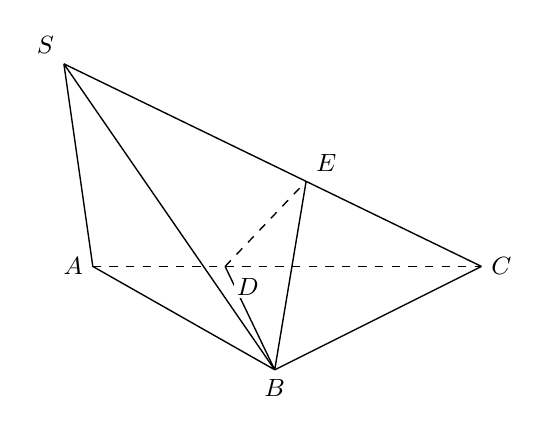
\begin{tikzpicture}[line width=.5pt,scale=1.05,font=\small]
  \coordinate (S) at (1.00,4.15);
  \coordinate (A) at (1.35,1.70);
  \coordinate (C) at (6.05,1.70);
  \coordinate (B) at (3.55,0.45);
  \coordinate (D) at (2.95,1.70);
  \coordinate (E) at (3.93,2.73);
  % 可见棱。
  \draw (S)--(A) (S)--(B) (S)--(C) (A)--(B) (B)--(C);
  % 底面被遮挡的棱 AC，以及截面内的 DE。
  \draw[dashed] (A)--(C);
  \draw[dashed] (D)--(E);
  % 截面 BDE 与底面的交线 BD、截面与面 SBC 的交线 BE。
  \draw (B)--(D) (B)--(E);
  \node[above left] at (S) {$S$};
  \node[left] at (A) {$A$};
  \node[below] at (B) {$B$};
  \node[right] at (C) {$C$};
  \node[fill=white,inner sep=1pt,below right=3pt] at (D) {$D$};
  \node[above right] at (E) {$E$};
\end{tikzpicture}
\end{center}
\nopagebreak[4]
\Needspace{4\baselineskip}
\textbf{解析}

\Needspace{5\baselineskip}
（1）由 $SA\perp$ 底面 $ABC$，$BC\subset$ 底面 $ABC$，得 $SA\perp BC$；又 $AB\perp BC$，$SA\cap AB=A$，故

\nopagebreak[4]
\[
BC\perp\text{\text{平面} }SAB,
\]

从而 $BC\perp SB$。

\Needspace{5\baselineskip}
在直角三角形 $SBC$ 中，

\nopagebreak[4]
\[
SB=\sqrt{SA^2+AB^2}=\sqrt2 a,\qquad BC=\sqrt2 a,
\]

故 $SB=BC$，$\triangle SBC$ 为等腰三角形。又 $DE$ 垂直平分 $SC$，$E$ 为 $SC$ 中点，故 $BE\perp SC$（等腰三角形底边中线即高）。

\Needspace{5\baselineskip}
于是 $SC\perp BE$，$SC\perp DE$，而 $BE\cap DE=E$，$BE$、$DE\subset$ 平面 $BDE$，所以

\nopagebreak[4]
\[
SC\perp\text{\text{平面} }BDE.
\]

（2）由（1）$SC\perp$ 平面 $BDE$，故平面 $BDE$ 的法向量可取 $SC$ 方向；平面 $BDC$ 即底面 $ABC$，其法向量垂直于底面。两平面所成角等于两法向量所成角。

\Needspace{5\baselineskip}
$SA\perp$ 底面，故 $SC$ 在底面上的射影为 $AC$，$SC$ 与底面所成角为 $\angle SCA$。在直角三角形 $SAC$ 中，

\nopagebreak[4]
\[
AC=\sqrt{AB^2+BC^2}=\sqrt{a^2+2a^2}=\sqrt3 a,
\]

\nopagebreak[4]
\[
\operatorname{tg}\angle SCA=\frac{SA}{AC}=\frac{a}{\sqrt3 a}=\frac{\sqrt3}{3},
\]

故 $\angle SCA=30^\circ$。于是 $SC$ 与底面法向量的夹角为 $90^\circ-30^\circ=60^\circ$，即面 $BDE$ 与面 $BDC$ 所成的二面角为 $60^\circ$。

\gkanswer{答案：卷内未列结果，仅注「见理工农医类第二卷第二题解答」。（1）为证明题；（2）二面角为 $60^\circ$（此值据题面推得，非卷内所载，见解析）。}

\end{answer}
\begin{answer}
\gksolhead{29}{}

\textbf{题目}：

（本题满分 14 分）

已知椭圆的焦点为 $F_1(-1,0)$ 和 $F_2(1,0)$，直线 $x=4$ 是椭圆的一条准线。

（1）求椭圆的方程；

（2）又设点 $P$ 在椭圆上，且 $|PF_1|-|PF_2|=1$，求 $\cos\angle F_1PF_2$ 的值。

（源疑点：卷面此式两端的绝对值符号磨损，仅有单竖线，按所见录为 $|PF_1|-|PF_2|=1$；无论是否取外绝对值，本题所求余弦值不变。）

\Needspace{4\baselineskip}
\textbf{解析}

\Needspace{5\baselineskip}
（1）设椭圆半长轴为 $a$，半焦距为 $c$。由焦点 $F_1(-1,0)$、$F_2(1,0)$ 得 $c=1$，中心在原点、长轴在 $x$ 轴上。准线 $x=\dfrac{a^2}{c}=4$，故 $a^2=4$，$a=2$，

\nopagebreak[4]
\[
b^2=a^2-c^2=4-1=3.
\]

\Needspace{5\baselineskip}
椭圆方程为

\nopagebreak[4]
\[
\frac{x^2}{4}+\frac{y^2}{3}=1.
\]

\Needspace{5\baselineskip}
（2）设 $r_1=|PF_1|$，$r_2=|PF_2|$。由椭圆定义 $r_1+r_2=2a=4$，又题设 $|r_1-r_2|=1$，故

\nopagebreak[4]
\[
r_1r_2=\frac{(r_1+r_2)^2-(r_1-r_2)^2}{4}=\frac{16-1}{4}=\frac{15}{4}.
\]

\Needspace{5\baselineskip}
在 $\triangle F_1PF_2$ 中，$F_1F_2=2$，由余弦定理

\nopagebreak[4]
\[
\cos\angle F_1PF_2
=\frac{r_1^2+r_2^2-F_1F_2^2}{2r_1r_2}
=\frac{(r_1+r_2)^2-2r_1r_2-4}{2r_1r_2}
=\frac{16-\frac{15}{2}-4}{\frac{15}{2}}
=\frac35.
\]

\gkanswer{答案：卷内未列结果，仅注「见理工农医类第二卷第三题解答」。（1）椭圆方程为 $\dfrac{x^2}{4}+\dfrac{y^2}{3}=1$；（2）$\cos\angle F_1PF_2=\dfrac35$（此二值据题面推得，非卷内所载，见解析）。}

\end{answer}
\begin{answer}
\gksolhead{30}{}

\textbf{题目}：

（本题满分 14 分）

已知数列 $\{a_n\}$ 的前 $n$ 项和的公式 $S_n=\dfrac{\pi}{12}(2n^2+n)$。

（1）求证 $\{a_n\}$ 是等差数列，并求出它的首项和公差；

\Needspace{5\baselineskip}
（2）记 $b_n=\sin a_n\cdot\sin a_{n+1}\cdot\sin a_{n+2}$，求证：对任何自然数 $n$，都有

\nopagebreak[4]
\[
b_n=\frac{\sqrt2}{8}(-1)^{n-1}.
\]

（源疑点：卷面「并求出它的首项的公差」中「的」字疑为「和」之误，此处按文意录为「首项和公差」。）

\Needspace{4\baselineskip}
\textbf{解析}

\Needspace{5\baselineskip}
（1）当 $n\ge 2$ 时，

\nopagebreak[4]
\[
a_n=S_n-S_{n-1}
=\frac{\pi}{12}\left[(2n^2+n)-\left(2(n-1)^2+(n-1)\right)\right]
=\frac{\pi}{12}(4n-1).
\]

\Needspace{5\baselineskip}
又 $a_1=S_1=\dfrac{\pi}{12}(2+1)=\dfrac{\pi}{4}$，与上式在 $n=1$ 时的值 $\dfrac{3\pi}{12}=\dfrac{\pi}{4}$ 一致，故对一切自然数 $n$ 有

\nopagebreak[4]
\[
a_n=\frac{(4n-1)\pi}{12}.
\]

\Needspace{5\baselineskip}
于是

\nopagebreak[4]
\[
a_{n+1}-a_n=\frac{4\pi}{12}=\frac{\pi}{3}
\]

为常数，$\{a_n\}$ 是首项 $a_1=\dfrac{\pi}{4}$、公差 $d=\dfrac{\pi}{3}$ 的等差数列。

\Needspace{5\baselineskip}
（2）记 $\theta=a_n=\dfrac{(4n-1)\pi}{12}$，则 $a_{n+1}=\theta+\dfrac{\pi}{3}$，$a_{n+2}=\theta+\dfrac{2\pi}{3}$。由三倍角公式

\nopagebreak[4]
\[
\sin 3\theta=4\sin\theta\sin\left(\frac{\pi}{3}+\theta\right)\sin\left(\frac{\pi}{3}-\theta\right),
\]

\Needspace{5\baselineskip}
并注意 $\sin\left(\dfrac{\pi}{3}-\theta\right)=\sin\left(\dfrac{2\pi}{3}+\theta\right)$，得

\nopagebreak[4]
\[
b_n=\sin\theta\sin\left(\theta+\frac{\pi}{3}\right)\sin\left(\theta+\frac{2\pi}{3}\right)=\frac14\sin 3\theta.
\]

\Needspace{5\baselineskip}
而

\nopagebreak[4]
\[
3\theta=\frac{(4n-1)\pi}{4}=n\pi-\frac{\pi}{4},
\]

\Needspace{5\baselineskip}
故

\nopagebreak[4]
\[
\sin 3\theta=\sin\left(n\pi-\frac{\pi}{4}\right)=(-1)^{n-1}\sin\frac{\pi}{4}=\frac{\sqrt2}{2}(-1)^{n-1}.
\]

\Needspace{5\baselineskip}
代入得

\nopagebreak[4]
\[
b_n=\frac14\cdot\frac{\sqrt2}{2}(-1)^{n-1}=\frac{\sqrt2}{8}(-1)^{n-1}.
\]

\gkanswer{答案：卷内未列结果，仅注「见理工农医类第二卷第四题解答」。（1）$a_1=\dfrac{\pi}{4}$，公差 $d=\dfrac{\pi}{3}$；（2）为证明题（结论均据题面推得，非卷内所载，见解析）。}

\end{answer}